\chapter{Wykład 2. Metodologia zarządzania projektami w przedsiębiorstwie informatycznym}

\section{Model wybranego procesu}
% strona 43

\subsection*{Model procesu implementacji w projekcie informatycznym}

\begin{itemize}
\item \textbf{Właściciel procesu:} Project Manager.
\item \textbf{Cel procesu:} implementacja produktu zgodnie z dostarczonymi wymaganiami klienta według założonego planu zarządzania projektem.
\item \textbf{Wejście:} wymagania klienta - spisane podczas spotkań oczekiwania klienta wobec produktu, Plan zarządzania projektem – podział prac i czas ich realizacji, Projekt aplikacji – szkic implementowanego programu.
\item \textbf{Wyjścia:} kod źródłowy – implementacja aplikacji zgodna z wymaganiami klienta, Dokumentacja techniczna – słowny opis zaimplementowanych funkcjonalności.
\item \textbf{Zakres procesu:} Proces obejmuje przełożenie projektu aplikacji na kod źródłowy. Proces nie ma zastosowania gdy produktem dostarczanym klientowi ma być sam projekt aplikacji.
\item \textbf{Schemat procesu:} Rysunek~\ref{schematProcesuImplementacji}.
\item \textbf{Opis procesu:} Po otrzymaniu wymaganych dokumentów, rozpoczyna się proces implementacyjny. Składa się on z dwóch czynności: implementacji oraz sporządzenia dokumentacji technicznej. Efektem tych czynności są kod źródłowy oraz dokumentacja.
\end{itemize}

\begin{figure}[!h]
\centering
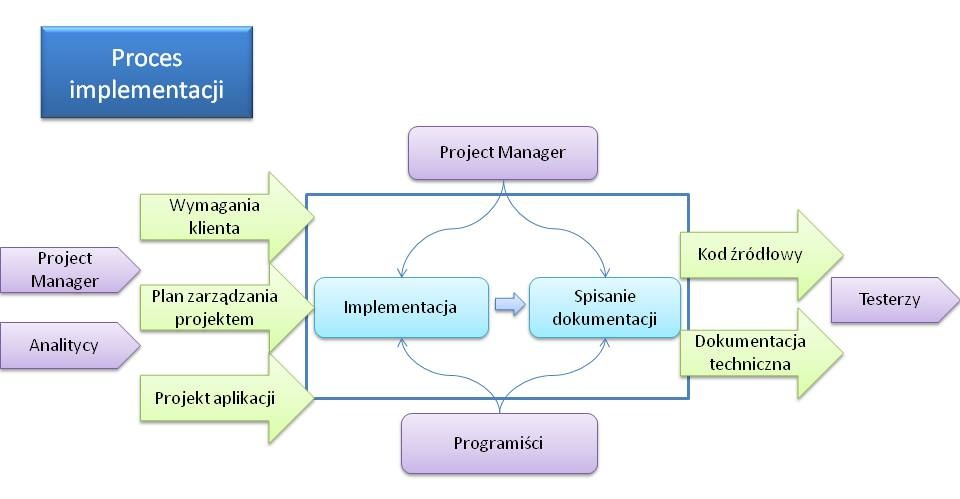
\includegraphics[width=\textwidth]{Prezentacja1}
\caption{Schemat procesu implementacji}
\label{schematProcesuImplementacji}
\end{figure}

% ===========================================================================

\section{Produkty, procesy, projekty}
% strona 78

\subsection*{Opis produktu}
Produktem wytwarzanym przez nasze przedsiębiorstwo jest system umożliwiający szybką i łatwą pracę związaną z zarządzaniem projektem informatycznym przy wykorzystaniu popularnej metodyki PMBOK. System będzie w pełni zgodny ze standardem PMBOK. Zostanie zaimplementowany przy wykorzystaniu architektury SOA. Podział na poszczególne moduły zostanie zrealizowany na dalszych etapach realizacji projektu.

\subsection*{Cykl życia produktu}
\begin{enumerate}
	\item Pomysł na produkt – inwestor zgłosił pomysł na opisany wcześniej produkt. Po dyskusji okazało się, że systemów wspomagających realizację projektów zgodnie z metodyką PMBOK jest aktualnie niewiele na rynku i napisanie takowego może się okazać dochodowych przedsięwzięciem.
	\item Opracowanie koncepcji – krok wymagający wielu spotkań z klientami w celu uzgodnienia i spisania oczekiwań wobec systemu i oszacowania przybliżonego czasu realizacji. Znając charakterystykę rynku oprogramowania IT ustalono, że czas realizacji projektu nie może przekroczyć 3 lat.
	\item Opracowanie projektu – stworzenie projektu implementowanego systemu zgodnie z uzgodnionymi z klientem wymaganiami.
	\item Implementacja i testy – najdłuższy krok zakładający implementację oraz testy powstałego w poprzednim etapie projektu aplikacji. Elementy wymagające dużych nakładów czasowych lub osobowych zostały oddelegowane do wykonania przez zewnętrznych podwykonawców (outsourcing).
	\item Dystrybucja – w trakcie implementacji inwestor pozyskiwał potencjalnych klientów oraz rozeznawał się w rynkach zbytu, na których nasz produkt mógłby się przyjąć.
	\item Sprzedaż – przy strategii sprzedaży nastawiliśmy się na długotrwały proces, poprzez ustalenie wysokiej ceny i nie promowanie nadmiernie produktu. Liczymy, że przedsiębiorstwa zadowolone z użytkowania naszego produktu rozreklamują go innym firmom pozyskując nam kolejnych klientów.
	\item Likwidacja – produkt będzie rozwijany do momentu, w którym przestanie to być opłacalne. Wtedy firma zakończy wszelkie prace nad tym produktem, jednak jego poprzednie wersje nie zostaną wycofane z rynku, ustanie jednak jakiekolwiek wsparcie przy ich użytkowaniu.
\end{enumerate}

\subsection*{Plan rozwoju produktu}
\begin{figure}[!h]
\centering
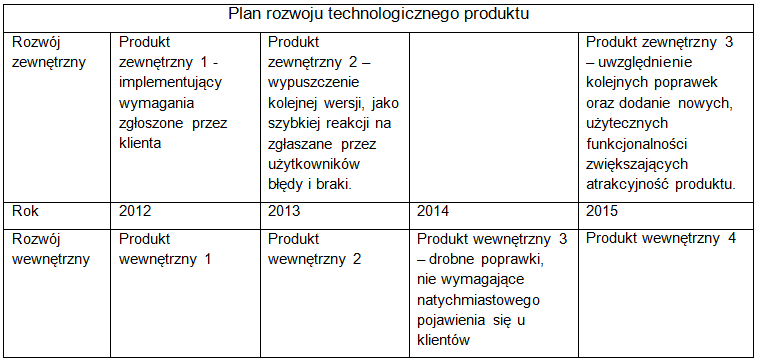
\includegraphics[width=\textwidth]{planRozwojuTechnologicznego}
\caption{Plan rozwoju technologicznego}
\label{planRozwojuTechnologicznego}
\end{figure}

\subsection*{Procesy w projekcie}
Sukces produktu jest uzależniony od szeregu procesów realizowanych w ramach projektu. Najważniejsze z nich to analiza oraz projektowanie aplikacji. Im dokładniej i bardziej szczegółowo system będzie opisany tym mniej czasu zajmie jego implementacja oraz zmniejsza się ryzyko błędnej interpretacji wymagań, a tym samym wprowadzania zazwyczaj bardzo kosztownych zmian. Proces implementacji, od którego zależy powstanie produktu. Jego prawidłowa realizacja wymaga również odpowiednio zdefiniowanych procesów komunikacji, monitorowania i kontroli, zarządzania wykonaniem projektu, zintegrowanej kontroli zmian oraz konfiguracją. Ich realizację opisują odpowiednie plany przedstawione w dalszej części dokumentacji. Ostatnim etapem jest proces zamykania projektu, który polega na zakończeniu wszystkich działań w projekcie w celu jego formalnego zakończenia. Dzięki zastosowaniu listy kontrolnej Project Manager upewni się, że wszystkie podstawowe zagadnienia zostały zrealizowane przed zamknięciem projektu.

% ===========================================================================

\section{Podejścia przy wytwarzaniu produktu}
	W swoim projekcie zdecydowaliśmy się skorzystać z podejścia mieszanego, które łączy podejście adaptacyjne z pro aktywnym. Rozpoczęcie prac nad produktem uwzględnia identyfikację wymagań klienta, ale dodatkowo jest poszerzone o spisanie funkcjonalności, które zdaniem ekspertów w dziedzinie metodyki PMBOK będą przydatne, a wręcz niezbędne, w implementowanej aplikacji. W podejściu typowo pro aktywnym, wprowadzanie jakichkolwiek zmian w dalszych etapach realizacji projektu jest bardzo kosztowne. 

	W naszym przypadku, dzięki zastosowaniu architektury SOA, wprowadzane zmiany zazwyczaj ograniczą się do jednego modułu, dzięki czemu nie będą konieczne modyfikacje całości aplikacji, a implementowane zmiany nie wpłyną na działanie reszty systemu. Zmniejszy to czas wprowadzania zmian, jak również testowania, ponieważ wystarczy sprawdzić jedynie ten konkretny moduł. Również dzięki iteracyjnemu modelowi wytwarzania oprogramowania system będzie podatny na wprowadzanie zmian. Wypuszczenie działającej aplikacji zagwarantuje dochód i umożliwi kontynuowanie prac nad kolejnymi wersjami.


% ===========================================================================

\section{Role w przedsiębiorstwie zorientowanym na projekty}
% strona 90

\subsection*{Role w przedsiębiorstwie}
\begin{itemize}
\item Klient
\item Kierownik projektu
\item Inwestor
\item Właściciel produktu
\item Kierownik proesu
\item Analityk
\item Projektant
\item Deweloper
\item Tester
\item Ekspert dziedzinowy
\item Wdrożeniowiec
\end{itemize}

\subsection*{Podejście pro aktywne}
Niewiele informacji pochodzi od klienta, większość funkcjonalności systemu jest przewidywana przez ekspertów na podstawie zidentyfikowanych potrzeb ewentualnych użytkowników. Raz ustalony projekt rzadko ulega zmianom.

\begin{itemize}
\item Klient – określa ogólny zarys wymaganego produktu. Nie podaje szczegółowych wymaga, a jedynie funkcjonalności jakie chciałby mieć. Jest otwarty na sugestie realizujących projekt.
\item Kierownik projektu – zarządza realizacją projektu, dbając aby przebiegała zgodnie z przyjętym planem i budżetem w określonym czasie. Zapewnia, by spisane wymagania zostały zaakceptowane przez wszystkich ważnych interesariuszy przed przystąpieniem do implementacji.
\item Inwestor – odpowiedzialny za pozyskiwanie funduszy do realizacji projektu oraz zapewnienie odpowiedniej liczby zasobów.
\item Właściciel produktu – Określa kryteria powodzenia projektu oraz sposób ich pomiaru.
\item Kierownik proesu – koordynuje proces produkcyjny oraz nadzoruje proces w zakresie jakościowym, ilościowym oraz kosztowym. Odpowiada za realizację produkcji zgodnie dostarczoną na początku specyfikacją oraz nadzór nad bieżącą produkcją.
\item Analityk – analizuje dostarczone przez klienta szczątkowe wymagania oraz sytuację na rynku oprogramowania wspierającego realizację projektów zgodnie z metodyką PMBOK. Na tej podstawie lepiej rozumie potrzeby klientów i rekomenduje rozwiązania oraz funkcjonalności, które powinny zostać uwzględnione w implementowanej aplikacji.
\item Projektant – dostarcza projekt wysokiego poziomu uwzględniając sugestie umieszczone w analizach oraz opisuje podejście do budowania architektury, decyduje także jaka architektura jest odpowiednia do projektu oraz spełnia jego wymagania.
\item Deweloperzy – osoby odpowiedzialne za stworzenie aplikacji (implementację kodu) według dostarczonego projektu oraz zgodnie z określonymi wymaganiami. W razie potrzeby konsultują się z analitykami w celu wyjaśnienia wątpliwości.
\item Tester – sprawdza działanie aplikacji, raportując wszelkie pojawiające się błędy. Zwraca uwagę czy wszystkie funkcjonalności działają zgodnie z dostarczoną dokumentacją oraz wymaganiami określonymi w fazie projektowania aplikacji.
\item Ekspert dziedzinowy – posiada szeroką wiedzę w dziedzinie realizacji projektów zgodnie z metodyką PMBOK, którą wspiera analityków biznesowych w procesie analizy implementowanego systemu. Osoba dostarczona przez klienta, której zadaniem jest ułatwienie identyfikacji wszystkich funkcjonalności przydatnych użytkownikom aplikacji.
\item Wdrożeniowiec – opracowuje strategię oraz plan wprowadzania nowych produktów. Przeprowadza instalację, szkolenie nowych użytkowników oraz sprawuje nadzór nad wykorzystaniem aplikacji.
\end{itemize}

\subsection*{Podejście adaptacyjne}
System będzie realizował jedynie wymagania podane przez klienta, bez dodatkowych funkcjonalności, nawet jeśli wydają się one potrzebne. Implementacja produktu otwarta na zmiany i sugestie klienta w trakcie jego realizacji. Podejście stosowane, gdy nie są znane późniejsze wymagania do produktu, określane są tylko wymagania na najbliższy horyzont czasowy z możliwością wprowadzania zmian na późniejszych etapach realizacji projektu.
\begin{itemize}
\item Klient – dostarcza szczegółowych informacji na temat żądanego systemu, ale tylko częściowych, tych najpilniejszych. Określa konkretne wymagania, a w trakcie realizacji systemu dostarcza uwag i ewentualnych żądań zmian w aplikacji.
\item Kierownik projektu – zarządza realizacją projektu, dbając aby przebiegała zgodnie z przyjętym planem i budżetem w określonym czasie. Jest odpowiedzialny za akceptację przez najważniejszych interesariuszy wszystkich zgłaszanych wymagań w kolejnych etapach rozwoju produktu.
\item Inwestor – odpowiedzialny za pozyskiwanie funduszy do realizacji projektu oraz zapewnienie odpowiedniej liczby zasobów.
\item Właściciel produktu – Określa kryteria powodzenia projektu oraz sposób ich pomiaru. Akceptuje pojawiające się zmiany w zakresie projektu i dba o spełnienie wymagań klienta.
\item Kierownik proesu – koordynuje proces produkcyjny oraz nadzoruje proces w zakresie jakościowym, ilościowym oraz kosztowym. Odpowiada za realizację produkcji zgodnie z dostarczaną na bieżąco specyfikacją oraz sprawuje nadzór nad aktualną produkcją.
\item Analityk – analizuje dostarczone przez klienta wymagania oraz sytuację na rynku oprogramowania wspierającego realizację projektów zgodnie z metodyką PMBOK. Na tej podstawie lepiej rozumie potrzeby klientów i rekomenduje rozwiązania dla zgłoszonych wymagań. Proces powtarzany po każdej aktualizacji wymagań.
\item Projektant – dostarcza a później modyfikuje projekt wysokiego poziomu uwzględniając sugestie umieszczone w analizach oraz opisuje podejście do budowania architektury, decyduje także jaka architektura jest odpowiednia do projektu oraz spełnia jego wymagania.
\item Deweloperzy – osoby odpowiedzialne za stworzenie i modyfikacje aplikacji (implementację kodu) według dostarczanych projektów oraz zgodnie z określonymi wymaganiami.
\item Tester – sprawdza działanie aplikacji, raportując wszelkie pojawiające się błędy. Zwraca uwagę czy wszystkie funkcjonalności działają zgodnie z dostarczoną dokumentacją oraz wymaganiami klienta.
\item Ekspert dziedzinowy – posiada szeroką wiedzę w dziedzinie realizacji projektów zgodnie z metodyką PMBOK, którą wspiera analityków biznesowych w procesie analizy implementowanego systemu. Osoba dostarczona przez klienta, której zadaniem jest pomaganie przy przekładaniu wymagań klienta na aplikację.
\item Wdrożeniowiec – opracowuje strategię oraz plan wprowadzania nowych produktów. Przeprowadza instalację, szkolenie nowych użytkowników oraz sprawuje nadzór nad wykorzystaniem aplikacji.
\end{itemize}


